%% ------------------------------------------------------------------------- %%
\chapter{Telas OLED Flexíveis}
\label{cap:oled}

A tecnologia OLED é baseada na iluminação através da aplicação de eletricidade em moléculas organicas \cite{HSWOLED}, denominado    eletroluminescência, como mostra a imagem \ref{fig:oled_early_product}. A eletroluminescência foi inicialmente pesquisada por André Bernanose e colegas de trabalho em 1950 na Nancy-Université na França. Eles aplicaram alta tensão (AC) no ar para materias como a acridina laranja, depositada e dissolvida em filmes finos de celulose ou celofane. O mecanismo proposto era a excitação direta das moléculas do corante ou a excitação de seus elétrons \cite{WikipediaOLED}.\\

Em 1960, Martin Pope e colaboradores da Universidade de Nova York desenvolveram eletrodos injetáveis óhmicos de contato a partir de cristais orgânicos. Eles descreveram ainda os requisitos energéticos necessários (funções trabalho) para os eletrodos de contato injetados. Esses contatos são a base da injeção de carga em todos os dispositivos OLED modernos. O grupo de Pope também observou pela primeira vez {\bf eletroluminescência} de corrente contínua (DC) sob vácuo em um único cristal puro de antraceno e em cristais de antraceno embebidos com tetraceno em 1963, usando uma pequena área de eletrodo de prata em 400V \cite{WikipediaOLED}.\\

\begin{figure}[!ht]
  \centering
  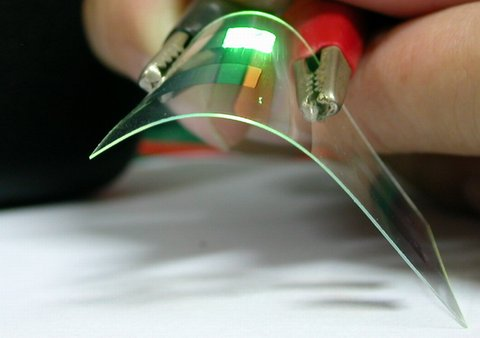
\includegraphics[width=.40\textwidth]{./figuras/oled_early_product} 
  \caption{Uma tela flexível OLED}
  \label{fig:oled_early_product} 
\end{figure}

OLED's são dispositivos solidos compostos composto por finas camadas de moléculas organicas que são capazes de criar eletricidade através da aplicação de eletricidade. OLED's podem prover imagens mais brilhantes, maior nitidez e consumindo menos elergia que suas antecessoras, LCD e LED \cite{HSWOLED}.\\

O OLED é um dispositivo semi-condutor sólido de 100 a 500 nanometros de espessura, ou seja, aproximadamente 200 vezes mais fino que um fio de cabelo humano. OLED's podem ter de 2 a 3 camadas de material orgânico; sendo que a terceira camada ajuda no transporte de elétron do cátodo para a camada emissiva como é possível ver na figura \ref{fig:camadas_oled} \cite{HSWOLED}.\\

%% ------------------------------------------------------------------------- %%
\section{Origem}
\label{sec:origem}

Dr. Ching Tang e Steven Van Slyke são os dois pioneiros da tecnologia OLED - de fato podemos dizer que eles são os inventores da tecnologia OLED em 1987 na Eastman Kodak. Os dois escreveram o artigo \textit{Electroluminescent devices with improved cathodes} para um seminário e este tem sido citado em mais de 5000 publicações. Agora, os dois pioneiros foram incluidos no \textit{hall} da fama dos consumidores de eletronicos \cite{OLEDPioneers}. \\

\begin{figure}[!ht]
  \centering
  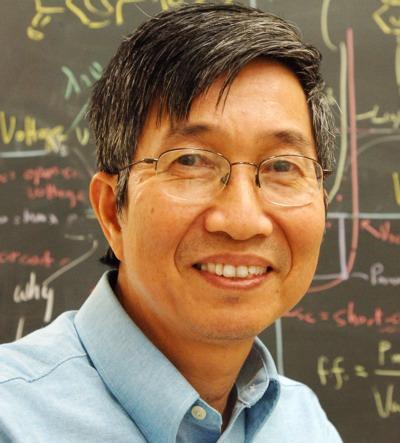
\includegraphics[width=.40\textwidth]{./figuras/ching_tang} 
  \caption{Criador da tecnologia OLED Ching Tang}
  \label{fig:ching_tang} 
\end{figure}

\begin{figure}[!ht]
  \centering
  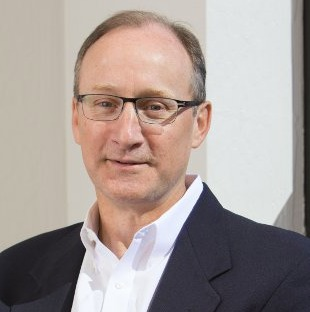
\includegraphics[width=.40\textwidth]{./figuras/steven_slyke} 
  \caption{Criador da tecnologia OLED Steven Van Slyke}
  \label{fig:steven_slyke} 
\end{figure}

Kodak lançou diversos dos primeiros dispositivos equipados com a tecnologia OLED, incluindo uma câmera digital com uma tela OLED de 2.2'' com 512 x 218 pixels \cite{WIOLEDT}.\\

No início dos anos 2000, pesquisadores do \textit{Pacific Northwest National Laboratory} e do Departamento de Energia inventou duas tecnologias necessárias para criar OLED\'s flexíveis (FOLED): a primeira, de vidro flexível um substrato de engenharia que fornece uma superfície flexível, e segundo, uma fina camada de proteção Barix que protege o OLED do aqucimento e ambientes úmidos \cite{WIOLEDT}.\\


%% ------------------------------------------------------------------------- %%
\section{Vantagens}
\label{sec:vantagens}

A tecnologia OLED possui algumas vantagens com relação as tecnologias de telas criadas anteriormente a ela. A seguir apresentamos a principais vantagens segundo diversos textos econtrados.

\begin{enumerate}
	\item[-] Maior brilho;
	\item[-] Imagens mais nítidas;
	\item[-] Utiliza menos energia que telas LCD e LED;
	\item[-] Maior ângulo visual sem distorção da imagem;
	\item[-] Taxa de atualização (\textit{frame rate}) de imagem maior;
	\item[-] Menor custo de fabricação.
\end{enumerate}

%% ------------------------------------------------------------------------- %%
\section{Composição e Fabricação}
\label{sec:composicao}

Tais como as tecnologias Plasma, LCD e LED, a tela OLED também possui algumas camadas em sua composição como mostra a figura \ref{fig:camadas_oled}, a seguir é apresentado quais são estas camadas e para que serve cada uma \cite{HSWOLED}. \\

\begin{figure}[!ht]
  \centering
  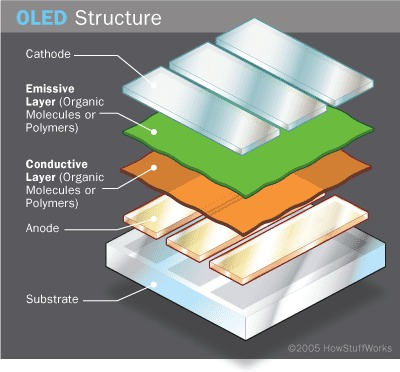
\includegraphics[width=.40\textwidth]{./figuras/camadas_oled} 
  \caption{Componentes OLED}
  \label{fig:camadas_oled} 
\end{figure}


%% ------------------------------------------------------------------------- %%
\subsection{Substrato (\textit{Substrate})}
\label{sec:substrato}

Produzido a partir de plástico transparente, vidro ou folha metálica possui a função de suportar o OLED.


%% ------------------------------------------------------------------------- %%
\subsection{Anódio (\textit{Anode})}
\label{sec:anodo}

Sendo transparente, o anódio remove elétrons, ou seja, adiciona  ``buracos''  de elétrons, enquanto há corrente elétrica no dispositivo.


%% ------------------------------------------------------------------------- %%
\subsection{Camadas Orgânicas (\textit{Organic layers})}
\label{sec:camadasorganicas}

Estas camadas são feitas de moléculas organicas ou polímeros, sendo que os tipos de moléculas e polímeros são diferentes entre as camadas.\\

{\bf Camada Condutiva:} Esta camada é feita de moléculas orgânicas plásticas que transportam os ``buracos'' do Anódio. Um polímero usado nesta camada é a polianilina.\\

{\bf Camada Emissiva:} Esta camada é feira de moléculas orgânicas plásticas, diferentes da camada Condutiva, e transporta elétrons do Catódio. É nesta camada onde a luz é gerada. Um dos polímeros usados nesta camada é o polifluoreno. 


%% ------------------------------------------------------------------------- %%
\subsection{Catódio (\textit{Cathode})}
\label{sec:catodio}

Pode ser ou não transparente, a depender do tipo de OLED. Esta camada injeta elétrons enquanto a corrente elétrica flui através do dispositivo. \\

O maior trabalho na construção de uma tela OLED é aplicar a camada orgânica ao substrato. Existem três maneiras de se fazer isso:

\begin{enumerate}
	\item {\bf Deposição a vácuo ou evaporação térmica a vácuo:} Em uma câmera de vácuo, as moléculas orgânicas são aquecidas suavemente (evaporadas) e é condensada como finas camadas sobre o substrato arrefecido. Este processo é caro e ineficiente.

	\item {\bf Deposição de vapor orgânico em fase:} Em baixa pressão, em uma câmera com paredes quentes, um gás portador transporta moléculas orgânicas evaporadas para o substrato resfriado, onde se condensam em finas camadas. Utilizar um gás portador aumenta a eficiência e reduz o custo de fabricação de OLED's.

	\item {\bf Impressão a jato de tinta:} Com a tecnologia de jato de tinta, os OLED's são pulverizados sobre substratos como tintas são pulverizadas no papel durante a impressão. A tecnologia jato de tinta reduz muito o custo de produção de OLED e permite que eles sejam impressos em grandes camadas de substrato para grandes telas, como telas de TV de 80 polegadas ou painéis eletrônicos.
\end{enumerate}


%% ------------------------------------------------------------------------- %%
\section{Funcionamento}
\label{sec:funcionamento}

\begin{figure}[!ht]
  \centering
  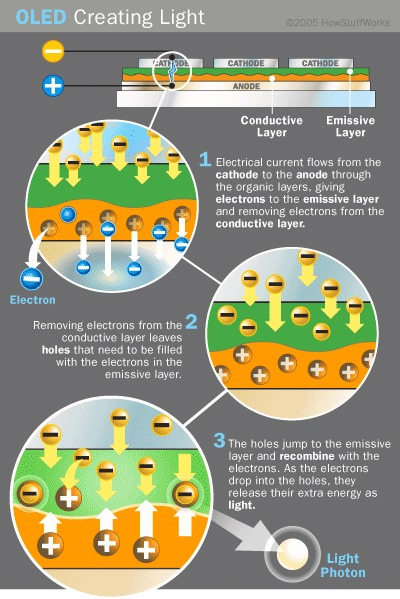
\includegraphics[width=.40\textwidth]{./figuras/oled-process} 
  \caption{Processo de geração de luz em telas OLED}
  \label{fig:oled-process} 
\end{figure}

Os OLED's emitem luz de um modo similar aos LED's, através de um processo chamado {\bf eletrofosforescência} descrito a seguir. 

\begin{enumerate}
	\item A bateria ou fonte de alimentação do dispositivo contendo o OLED aplica uma voltagem na tela OLED. 

	\item Uma corrente elétrica é passada do cátodo para o anódio através das camadas orgânicas. O cátodo fornece elétrons à camada emissiva das moléculas orgânicas. O anódio remove elétrons da camada condutora de moléculas orgânicas (isso é o equivalente a dar buracos de elétrons para a camada condutora).

	\item Na fronteira entre a camada emissiva e as camadas condutoras, os elétrons encontram ``buracos'' de elétrons. Quando um elétron encontra um ``buraco'' de elétron, ele preenche o buraco (ele cai no nível de energia do átomo que perdeu um elétron). Quando isso acontece, o elétron fornece energia na forma de um fóton de luz. 

	\item O OLED emite luz. 

	\item A cor da luz depende do tipo de molécula orgânica na camada emissora. Os fabricantes colocam vários tipos de filmes orgânicos no mesmo OLED para fazer displays coloridos.

	\item A intensidade ou brilho da luz depende da quantidade de corrente elétrica aplicada: quanto maior a corrente, maior o brilho da luz.
\end{enumerate}

Os tipos de moléculas usados pelos ciêntistas da Kodak em 1987 nas primeiras OLED's foram moléculas orgânicas pequenas. Sobretudo, essas moléculas luzes brilhantes sendo necessário utilizar o processo de depósito a vácuo (muito caro e ineficiênte) para colocá-la no substrato. \\

Desde 1990, pesquisadores tem usado polímeros grandes para emitir luz. Polímeros podem ser menos dispendiosos e ser aplicados em grandes telas, tornando-se mais adequados para monitores de tela grande \cite{HSWOLED}.\\


%% ------------------------------------------------------------------------- %%
\section{Tipos de telas OLED}
\label{sec:tipos}

Existem diversos tipos de telas OLED conforme listado a seguir \cite{HSWOLED}. Este trabalho no entanto, aborda mais detalhadamente os OLED flexíveis (FOLED).

\begin{enumerate}
	\item OLED de Matriz Passiva (POLED)
	\item OLED de Matriz Ativa (AMOLED)
	\item OLED Transparente 
	\item \textit{Top-Emitting} OLED 
	\item OLED dobráveis (FOLED)
	\item OLED Branca 
\end{enumerate}


%% ------------------------------------------------------------------------- %%
\section{Samsung Galaxy Round e LG G Flex}
\label{sec:devicesnomercado}

No final de 2013 a Samsung lançou no mercado o primeiro dispositivo com tela Super-AMOLED curva, o Galaxy Round mostrado na figura \ref{fig:galaxy-round}. Com tela de 5.7 polegadas, 154 gramas e 7.9mm de espessura, sua tela tem uma curvatura angular de 400mm \cite{NOLEDDN}.\\

\begin{figure}[!ht]
  \centering
  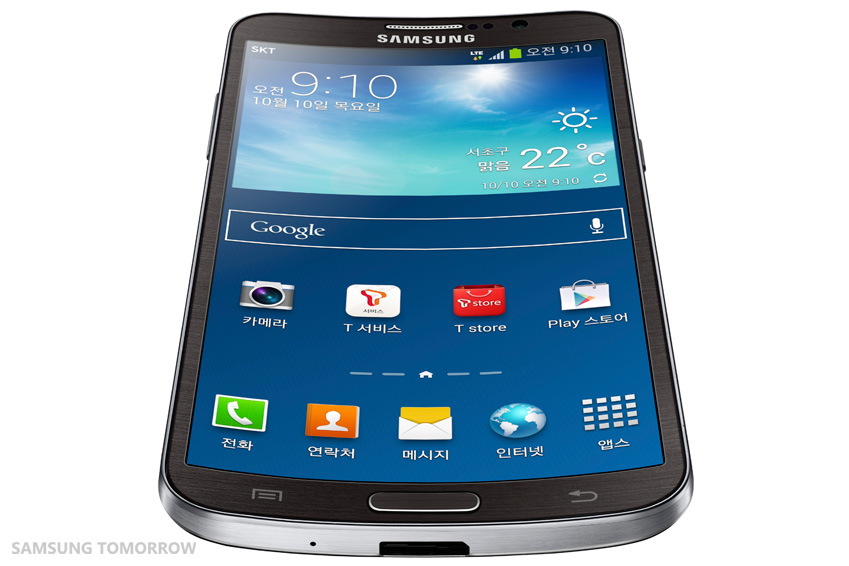
\includegraphics[width=.60\textwidth]{./figuras/galaxy-round} 
  \caption{Samsung Galaxy Round}
  \label{fig:galaxy-round} 
\end{figure}

Também no fim de 2013, logo após o lançamento realizado pela Samsung, a LG lançou sua versão de dispositivo curvo, o LG G Flex (figura \ref{fig:g-flex}). Com 6 polegadas e tela OLED com substrato de plástico de 1280 x 70 pixels de resolução, com apenas 0.44mm de espessura e 700mm de curvatura angular.\\

\begin{figure}[!ht]
  \centering
  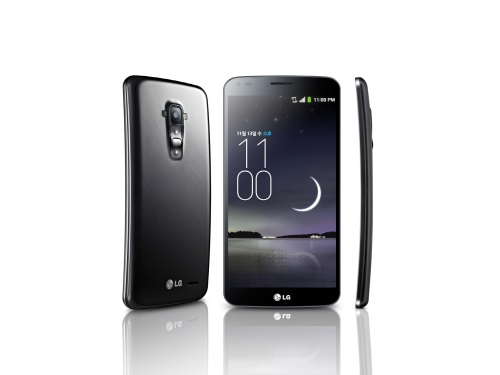
\includegraphics[width=.70\textwidth]{./figuras/g-flex} 
  \caption{LG G Flex}
  \label{fig:g-flex} 
\end{figure}

No entanto, se há telas flexíveis, também são necessários outros componentes com esta mesma característica. Desta forma, a LG Chem’s Stack \& Folding e outras empresas apresentaram um protótipo de bateria flexível que pode ser vista em um dispositivo na figura \ref{fig:flexible-battery} a seguir \cite{NOLEDDN}.\\

\begin{figure}[!ht]
  \centering
  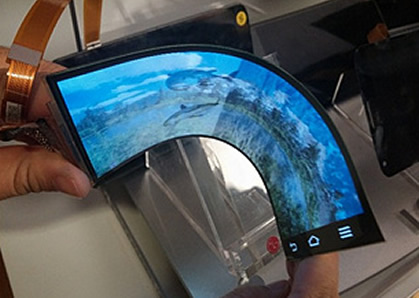
\includegraphics[width=.80\textwidth]{./figuras/flexible-battery} 
  \caption{Dispositivo Móvel com bateria Flexível}
  \label{fig:flexible-battery} 
\end{figure}


%% ------------------------------------------------------------------------- %%
\section{Investimento em telas Flexíveis}
\label{sec:investimento}

A tecnologia \textit{Flexible} OLED irá mexer com as indústrias de celulares, tablets e PC. As empresas que não adotarem serão passadas para trás e as empresas que já fazem saem na frente. Esta tela flexível, em breve, será encontrada em quase todos os dispositivos com telas sejam eles móveis ou não \cite{FSIJS}.\\

Há tempos ocorreu a substituição natural dos dispositivos móveis com botões físicos por dispositivos móveis sensíveis ao toque. Semlhante a este movimento, no futuro próximo poderá acontecer com dispositivos móveis ou não, com telas convencionais e dispositivos, móveis ou não, com telas flexíveis \cite{FSIJS}.\\

\begin{figure}[!ht]
  \centering
  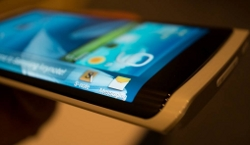
\includegraphics[width=.70\textwidth]{./figuras/oled-samsung-device} 
  \caption{Protótipo da Samsung com tela flexível}
  \label{fig:oled-samsung-device} 
\end{figure}

Tela com a tecnologia FOLED podem ser enroladas em um tubo para facilitar o transporte ou usado como pulseiras, relógios e outros acessórios do cotidiano. A tecnologia pode criar uma experiência de visualização mais panorâmica sobre televisões curvas e pode até mesmo ser usado como papel virtual. Estas são apenas algumas aplicações destas telas dobráveis que estão começando a surgir, e considerando que flexibilidade não é o único benefício que o OLED traz \cite{FSIJS}.\\

Além da flexibilidade, estas telas oferecem maior leveza, baixo consumo de energia, e é uma alternativa mais resistênte para telas sensíveis ao toque convencionais. Isso significa que ter dispositivos mais finos e leves, com telas maiores e maior vida útil da bateria. E isso para não mencionar as resoluções possíveis que são enormes, maior contraste e tempo de resposta mais rápido. Telas de OLED flexíveis já chegaram ao mercado de televisões curvas. Eles são incrivelmente finas e absolutamente linda aos olhos \cite{FSIJS}:\\

\begin{figure}[!ht]
  \centering
  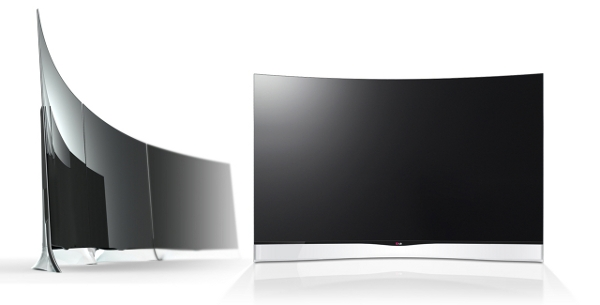
\includegraphics[width=.70\textwidth]{./figuras/flexible-tv} 
  \caption{Televisão com Tela Flexível}
  \label{fig:flexible-tv} 
\end{figure}

UBI Research acredita que o mercado de telas OLED flexíveis/dobráveis será de 700 milhões de dólares em 2014 e de 15 bilhões de dólares em 2018! IHS Display Bank, a indústria global de telas flexíveis, também verá um crescimento dramático e tornar-se um mercado de US\$ 1,5 bilhão em 2016 e irá superar US\$ 10 bilhões em 2019! \cite{NOLEDDN}.\\

No momento temos duas grandes empresas competindo por este mercado, são elas Samsung e LG.\\

A Samsung desenvolveu sua própria tecnologia de telas flexíveis baseada na tecnologia OLED e chamou-a de YOUM \cite{SYOUM}. A LG planeja aumentar sua linha de produção de telas flexíveis nos próximos anos. A LG acredita que 12\% de todos os \textit{smartphones} no mundo serão curvados, flexíveis ou dobráveis em 2015, acredita-se que até 2018 este número seja de 40\%.\\


%% ------------------------------------------------------------------------- %%
\section{Futuro de telas OLED Flexíveis}
\label{sec:futuro}

Pelo fato de telas flexíveis OLED serem extremamente finas e leves, elas podem ser usadas para criar telas flexíveis e até mesmo transparentes. Algo bem intrigante pois abre um mundo de possibilidades, como \cite{OIBOI}: 

\begin{enumerate}
    \item[-] Telas curvas colocadas em superfícies não planas;
    \item[-] Dispositivos vestíveis com OLED;
    \item[-] Telas de OLED transparentes embutidas em janelas;
    \item[-] Telas OLED em pára-brisas de automóveis;
    \item[-] Novos projetos para lâmpadas;
    \item[-] E muitos mais que não podemos sequer imaginar hoje!
\end{enumerate}

Diversar empresas estão voltando seus esforços com pesquisa e desenvolvimento a cerca desta tecnologia. \\

A seguir é apresentado uma série de imagens que representam de forma visual algumas ideias que se tem da aplicação de telas OLED flexíveis, ou simplesmente, FOLED, e também não flexíveis.\\

\begin{figure}[!ht]
  \centering
  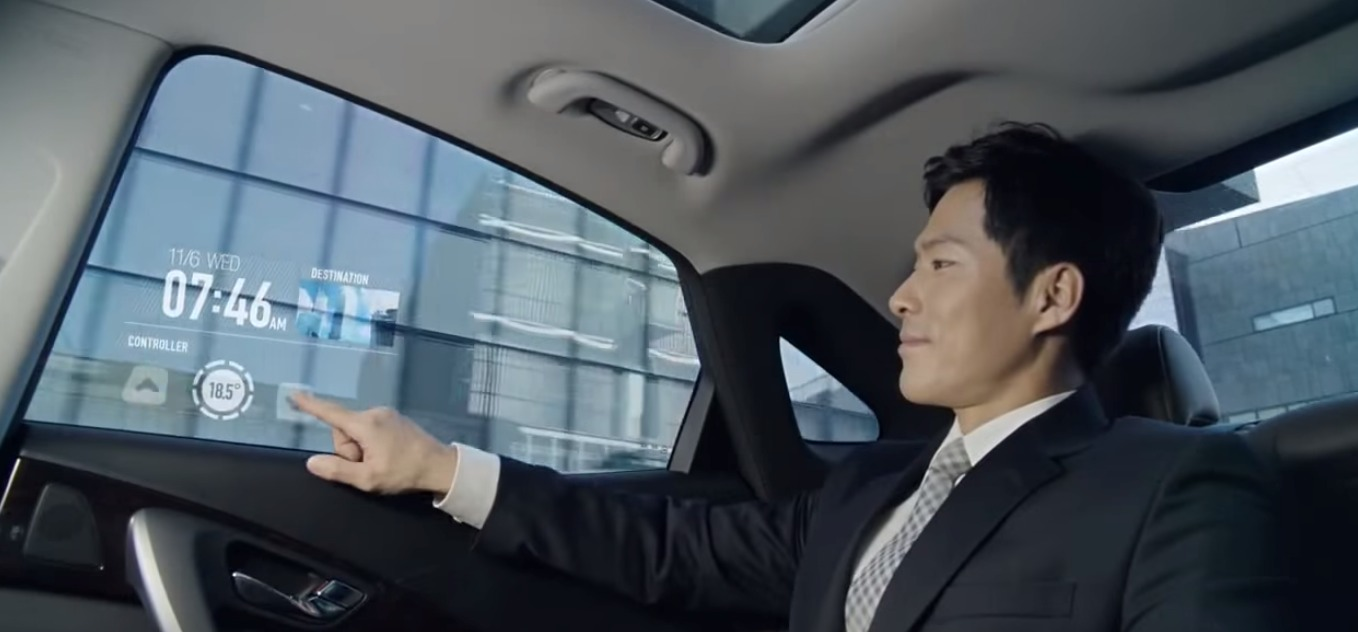
\includegraphics[width=.90\textwidth]{./figuras/oled-future1} 
  \caption{Tela OLED na janela do Carro}
  \label{fig:oled-future1} 
\end{figure}

\begin{figure}[!ht]
  \centering
  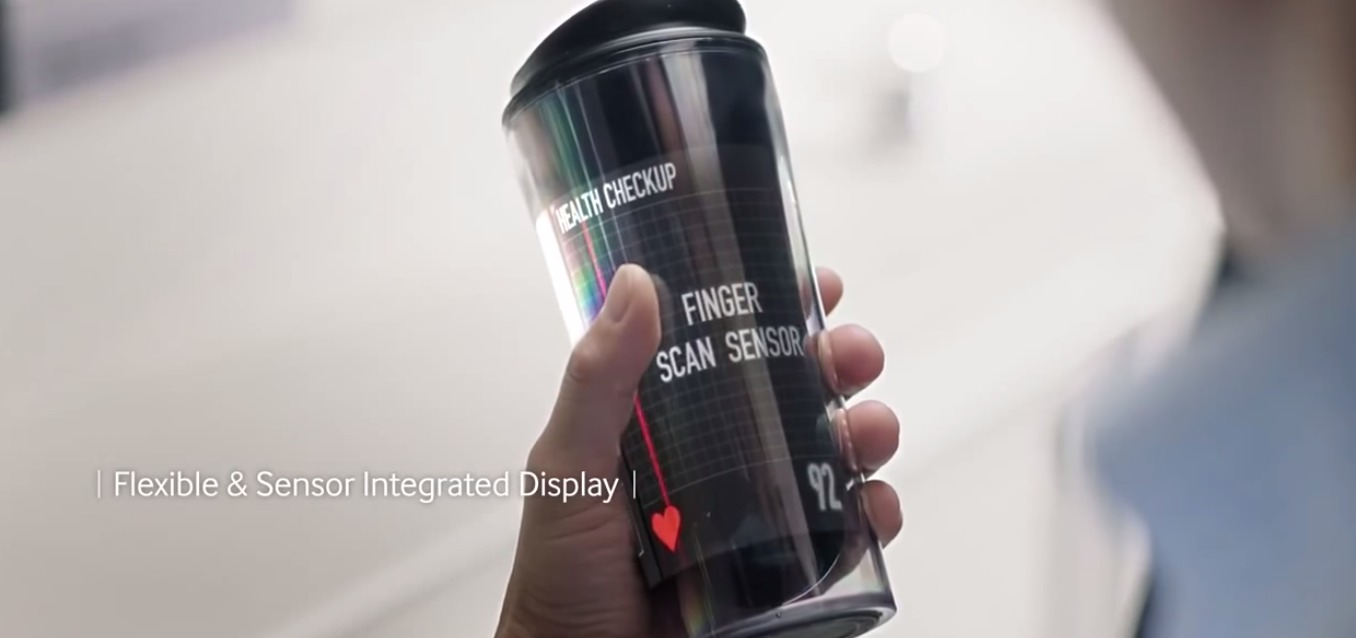
\includegraphics[width=.90\textwidth]{./figuras/oled-future2} 
  \caption{Tela OLED no copo}
  \label{fig:oled-future2} 
\end{figure}

\begin{figure}[!ht]
  \centering
  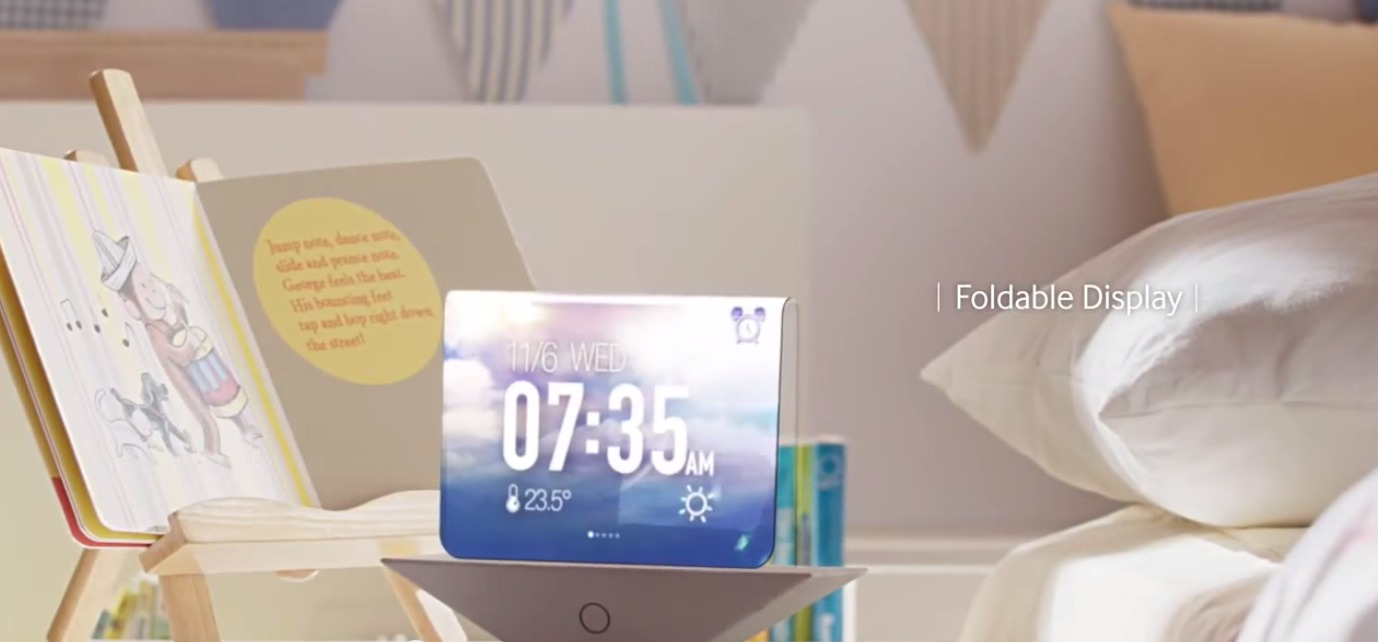
\includegraphics[width=.90\textwidth]{./figuras/oled-future3} 
  \caption{Tela Flexível}
  \label{fig:oled-future3} 
\end{figure}

\begin{figure}[!ht]
  \centering
  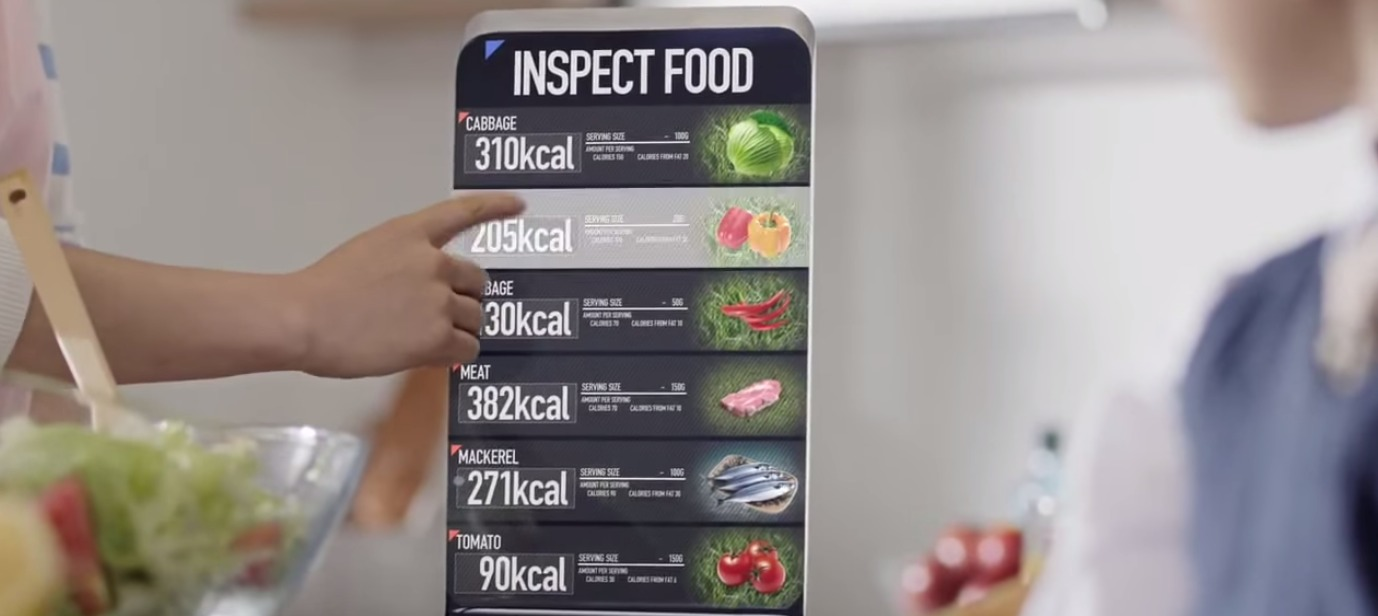
\includegraphics[width=.90\textwidth]{./figuras/oled-future4} 
  \caption{Tábua de carne com tela OLED com informações de nutrição na tela}
  \label{fig:oled-future4} 
\end{figure}

\begin{figure}[!ht]
  \centering
  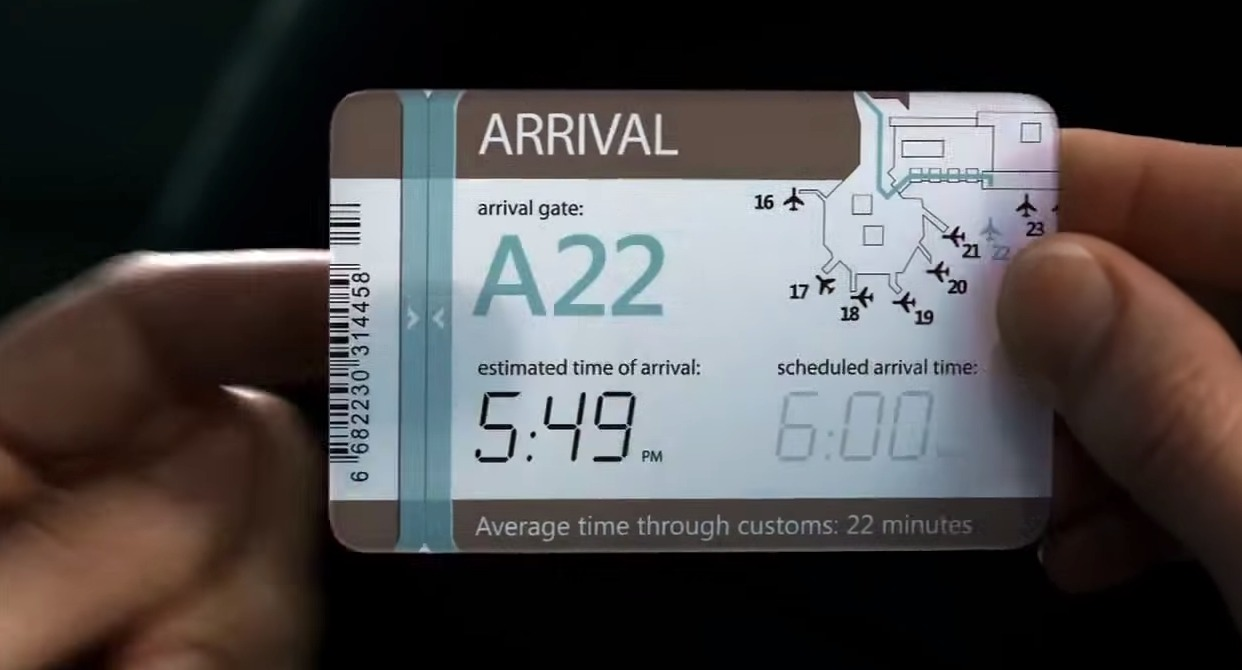
\includegraphics[width=.90\textwidth]{./figuras/oled-future5} 
  \caption{Ticket aéreo OLED}
  \label{fig:oled-future5} 
\end{figure}

\begin{figure}[!ht]
  \centering
  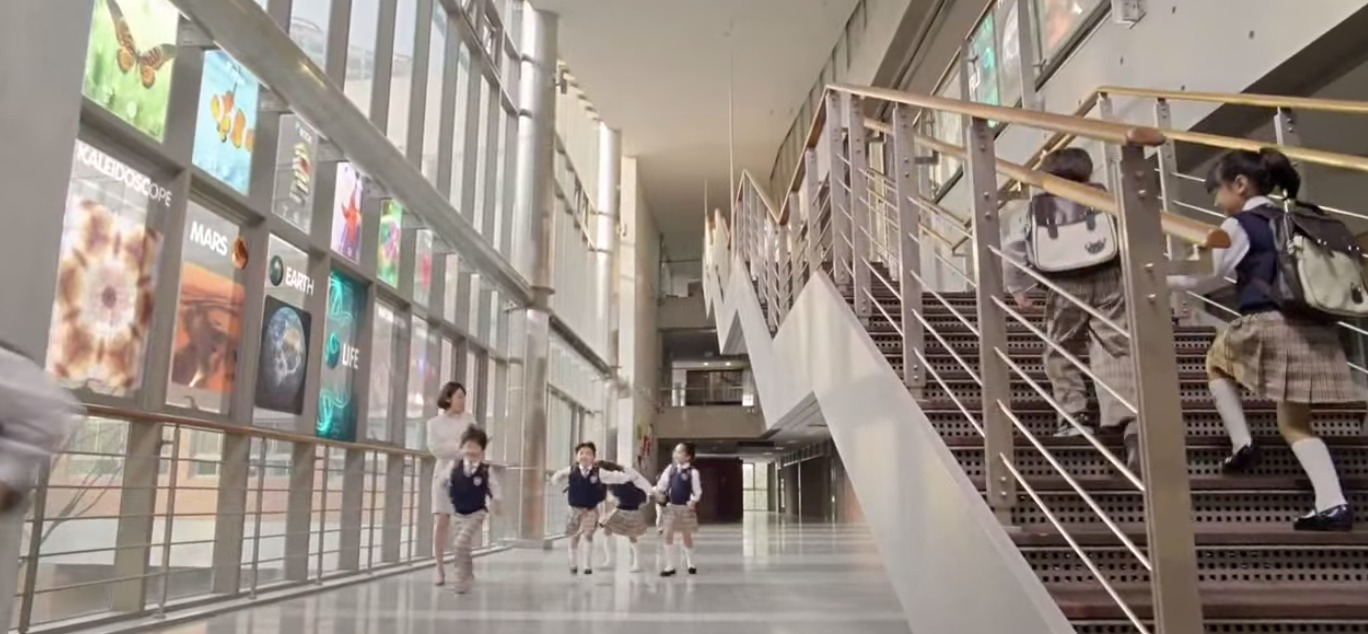
\includegraphics[width=.90\textwidth]{./figuras/oled-future6} 
  \caption{Janelas OLED}
  \label{fig:oled-future6} 
\end{figure}

\begin{figure}[!ht]
  \centering
  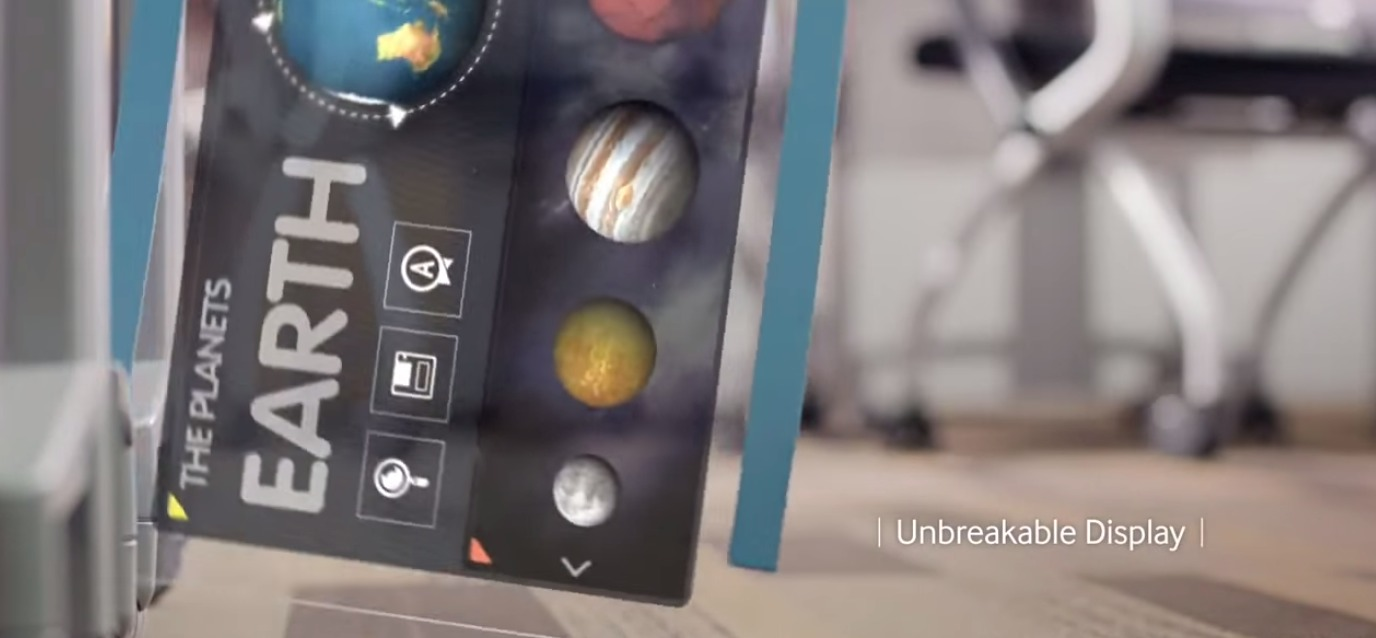
\includegraphics[width=.90\textwidth]{./figuras/oled-future7} 
  \caption{Telas OLED são mais resistentes}
  \label{fig:oled-future7} 
\end{figure}

\begin{figure}[!ht]
  \centering
  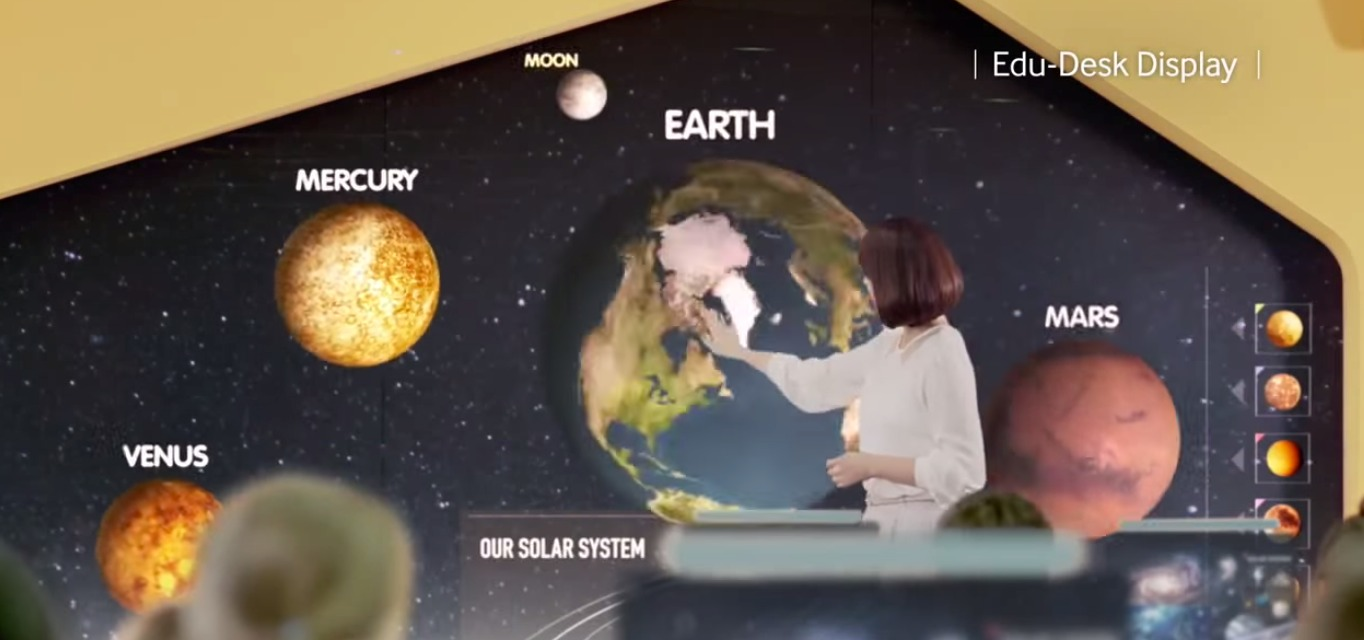
\includegraphics[width=.90\textwidth]{./figuras/oled-future8} 
  \caption{Telas OLED para educação}
  \label{fig:oled-future8} 
\end{figure}
